\subsection{Mechanik}

\subsubsection{Schussvorrichtung}
Die Hauptaufmerksamkeit zu Beginn gilt dem Prozess des Schiessens/ Befördern 
der Bälle. Aus diesem Grund wird entschieden, einen Versuchsaufbau zu 
konstruieren, um diese Funktion auf ihre Zuverlässigkeit und Genauigkeit zu 
testen. Als erstens wird ein Aufbau hergestellt, welcher die Bälle mit Hilfe 
eines Rades beschleunigt. \\
%
Die Konstruktion besteht hauptsächlich aus Holz, das es dadurch relativ 
einfach ist Anpassungen vorzunehmen. Die Lagerung der Welle mit welcher das 
Rad aus dem Modellbau dreht, wird mit zwei im Holz eingepressten Kugellagern 
realisiert. Da die berechnete Drehzahl des Rades zwischen 700 U/min bis 900 
U/min liegt, muss ein passender Motor gefunden werden. Motoren in diesem 
Drehzahlbereich sind jedoch sehr rar. Aus diesem Grunde wird auf einen Motor 
welcher bei RC-Modellautos eingesetzt wird zurückgegriffen. Dieser hat jedoch 
eine Drehzahl von über 20'000 U/min und muss deshalb stark untersetzt werden, 
um die gewünschte Raddrehzahl zu erhalten. Die Untersetzung wird mit zwei 
Riemenscheiben und einem O-Ring gelöst. Dadurch wird eine Untersetzung von 
ca. 1:30 erreicht damit der Ball die richtige Abschussgeschwindigkeit erhält. 
Da dieser Motor leider einen relativ hohen Drehzahl Einbruch hat sobald ein 
Ball geschossen wird, muss nach einer Alternative gesucht werden. Der 
zweite Motor, mit welchem getestet wird, stammt aus dem Flugzeugmodellbau und 
ist ein Brushless Innenläufer Motor mit Getriebe. Mit diesem können die 
Bälle in sehr kurzen Abständen mit nahezu gleich bleibender Drehzahl geschossen 
werden. Der Abschusswinkel bei diesen Versuchen wird experimentell ermittelt 
und mit ca. 50$^\circ$ als optimal festgelegt. \\
\begin{figure}[h!]          
	\centering             
	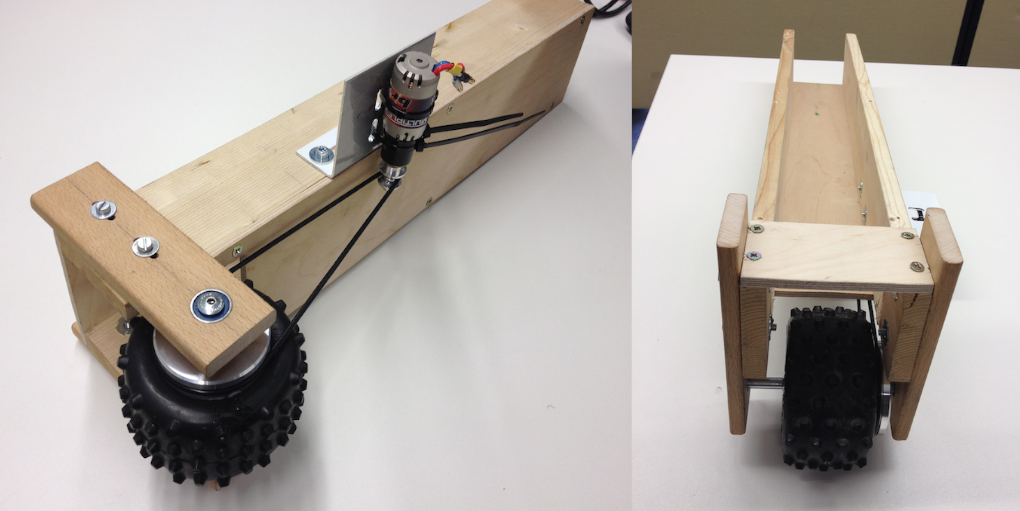
\includegraphics[width=0.8\textwidth]{fig/Schussvorrichtung.png}    
	\caption{Schussvorrichtung}
	
	\label{fig:Schussvorrichtung}
\end{figure}
\noindent
\\Anschliessend wird ein Mechanismus gesucht mit welchem die Bälle 
gleichmässig zum Beschleunigungsrad geführt werden können, damit die Wurfweite 
nicht beeinflusst wird. Die Idee ist es, mit einem umschlingenden Band die 
Bälle nacheinander zuzuführen. Beim Versuch wird als Band eine 0.1 mm dicke 
Präzisionsstahlfolie verwendet. Diese zeichnet sich durch eine hohe Stabilität, 
Aufrollbarkeit und ein geringes Gewicht aus. Beim Test ist das Band auf der 
einen Seite befestigt, umschlingt alle Tennisbälle und wird kurz vor dem Rad 
durch einen Schlitz im Holz nach draussen geführt. Leider kann bis heute 
diese Technik nur manuell getestet werden, was so viel bedeutet wie, das Band 
wird von Hand beim Test hinausgezogen. \\


\subsubsection{Drehvorrichtung}
Beim Test der Drehvorrichtung wurde darauf geachtet, dass genau diese Komponenten verwendet werden, welche auch für die Endlösung vorgesehen sind. Der ganze Versuch wurde daher auf einer 1/4 Zoll dicken Aluminium Platte aufgebaut. Als Antrieb diente ein Schrittmotor mit 200 Schritten (QSH 4218, QMot.eu). Die Übersetzung wurde mit zwei Zahnräder (z1=25 und z2=120) realisiert. Die Idee ist es, den Turm schlussendlich direkt auf dem grosse Zahnrad aufzubauen um weitere Komponenten zu sparen. Für die Lagerung welche ausschliesslich axiale Kräfte aushalten muss, wurden zwei UBC Bearing Axial-Rillenkugellager 51104 verwendet. Diese Lagerung ermöglicht das Drehen des grossen Zahnrades und zugleich ein spielfreies Einstellen, was für die Genauigkeit sehr entscheiden sein wird.
Der Test war erfolgreich da festgestellt wurde, dass erstens die Konstruktion genügend schnell arbeiten kann und zweitens ausreichen Kraft vorhanden ist um das Gewicht des Turms zu drehen.

\begin{figure}[h!]          
	\centering             
	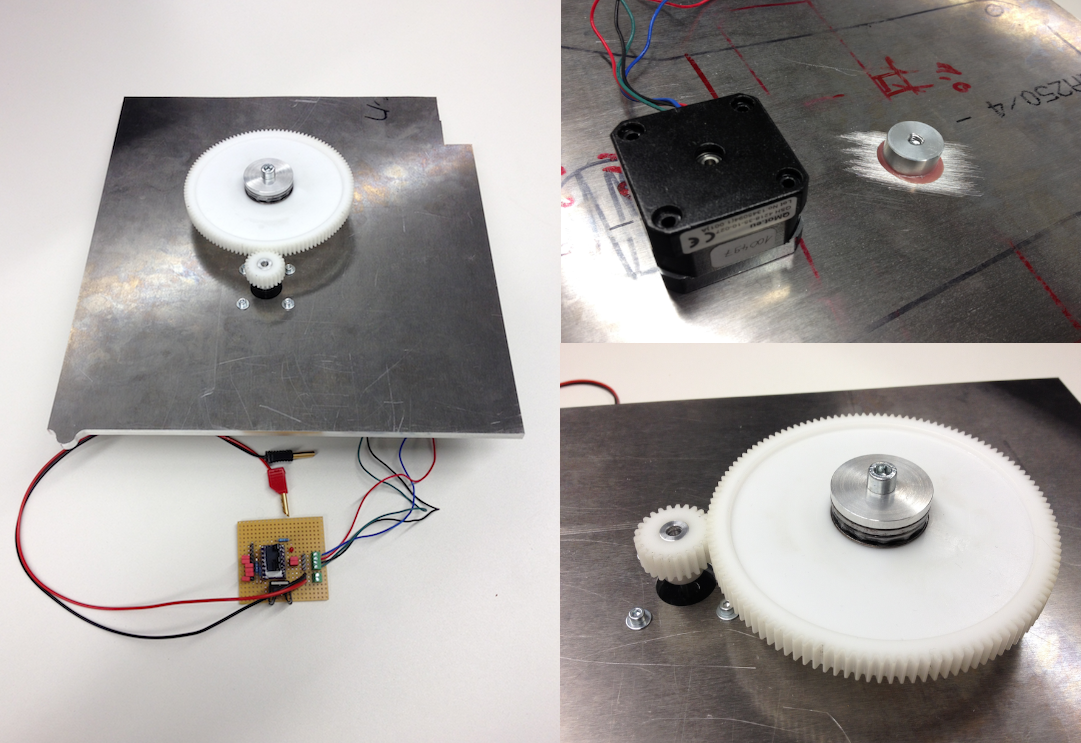
\includegraphics[width=0.8\textwidth]{fig/Drehvorrichtung.png}    
	\caption{Drehvorrichtung}
	
	\label{fig:Drehvorrichtung}
\end{figure}
\noindent



